Before AlphaGo, several extensions of MCTS had led to high-performance Go programs; \textit{Pachi}\cite{b29} and \textit{Feugo}\cite{b30} were the strongest in the open-source community, and \textit{Zen} and \textit{Crazy Stone}\cite{b31} were likewise in the commercial domain. The performance of the RL policy network was first evaluated by playing against Pachi. In contrast to the ones only based on supervised learning of DCNNs\cite{b32, b33}, it won 85\% of games against Pachi and 80\% against the SL policy network. Next, AlphaGo was evaluated against all the above programs in an internal tournament, including an additional open-source program \textit{GnuGo}, based on state-of-the-art search methods that preceded MCTS (cf. Fig.~\ref{Eval_AplhaGo}a). Programs were evaluated on an Elo scale \cite{b34}. All were allowed 5s of computation time per move. AlphaGo turned out to be many dan ranks stronger, winning 494 out of 495 games (99.8\%) against any previous Go programs. Games with four handicap stones were also played to provide a fair challenge to AlphaGo, and it won 77\%, 86\%, and 99\% of handicap games against Crazy Stone, Zen, and Pachi, respectively. Silver et al.\cite{b12} also developed a distributed version that won 77\% of games against single-machine AlphaGo and 100\% against other programs. 
\begin{figure}[t]
    \centering
    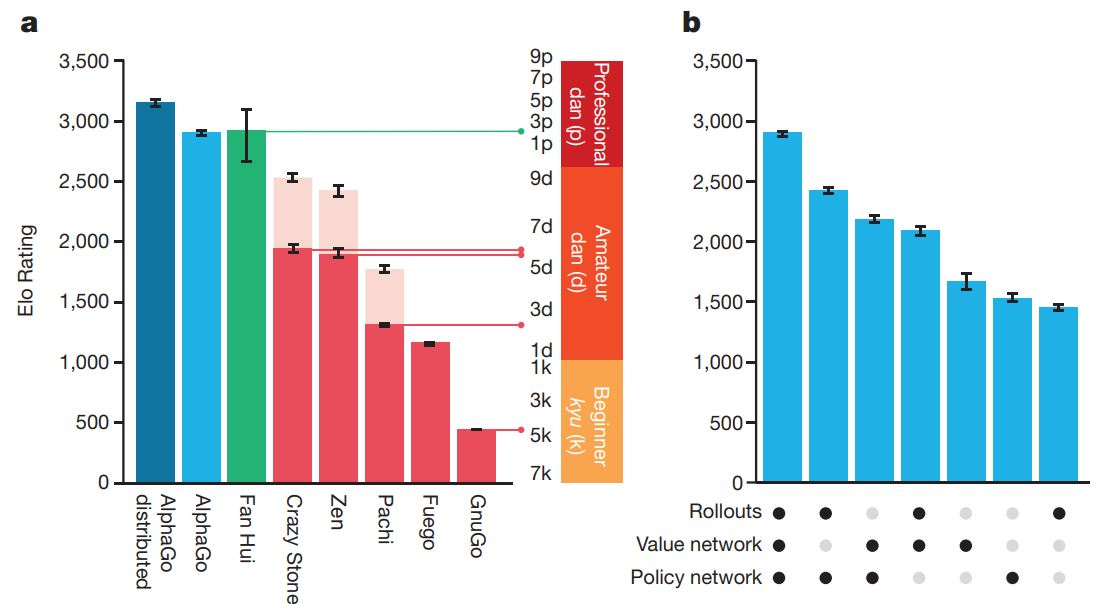
\includegraphics[width = 0.85\columnwidth]{Eval_1}
    \caption{Tournament evaluation of AlphaGo\cite{b12}}
    \label{Eval_AplhaGo}
\end{figure}
Other variants of AlphaGo (cf. Fig.~\ref{Eval_AplhaGo}b), e.g., using just the value network $(\lambda=0)$ exceeded the performance of all other Go programs, showing that value networks provide a viable alternative to Monte Carlo evaluation. However, the mixed version $(\lambda=0.5)$ performed best, winning $\geq$95\% of games against other variants. This combination of the two different position-evaluation methods is complementary: the value network approximates the outcome of games played by the strong but slow $p_\rho$, while the rollouts can precisely score and evaluate the outcome of games played by the weaker but faster rollout policy $p_\pi$.

% \subsection{Against expert human Go players}
AlphaGo (distributed version) was evaluated against three-time European Champion Mr. Fan Hui, a professional 2-dan Go player (in 2015). AlphaGo's win (5-0) was the first time a computer Go program defeated a human professional without a handicap. AlphaGo then competed against Mr. Lee Sedol, winner of 18 world titles (in 2016). AlphaGo's 4-1 victory was a landmark achievement a decade ahead of its time. AlphaGo thus earned a 9-dan professional ranking (highest rank), the first-ever accolade received by a computer Go program. In January 2017, an online version of AlphaGo called Master achieved 60 straight wins in time-control games against top international players. Four months later, Master took part in the Future of Go Summit in China, the birthplace of Go. Master defeated the Chinese grandmaster Mr. Ke Jie in a match (3-0). 